\documentclass[border=2]{standalone}
\usepackage{tikz}

\usetikzlibrary{arrows, arrows.meta}

\tikzset{
    larrow/.style={
        >={Triangle[left,length=6pt,width=4pt]},
        shorten >= 4pt, shorten <= 4pt,
        semithick,
        ->
    }
}

\newcommand{\halfedge}[2]
{
    \draw[larrow, transform canvas={yshift=1.5pt}] (#1) -- (#2);
    \draw[larrow, transform canvas={yshift=-1.5pt}] (#2) -- (#1);
}

\newcommand{\halfedges}[2]
{
    \draw[larrow, transform canvas={yshift=1pt}] (#1) -- (#2);
    \draw[larrow, transform canvas={yshift=-1pt}] (#2) -- (#1);
}

\begin{document}
    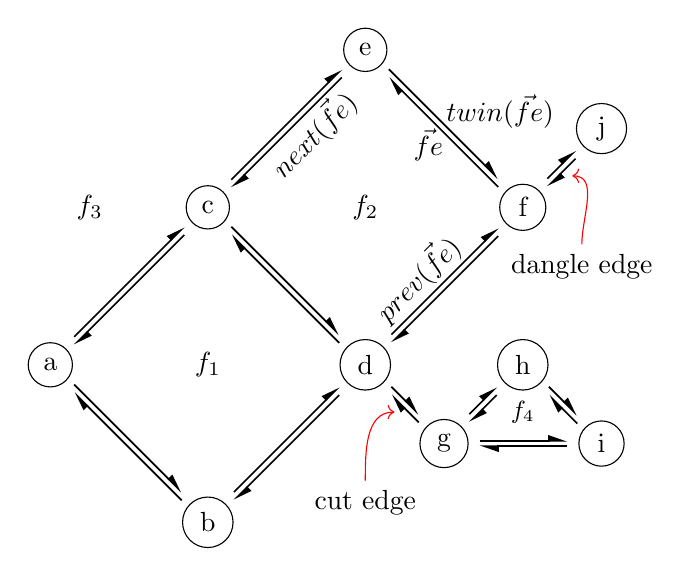
\begin{tikzpicture}
        \tikzstyle{node1}=[draw,shape=circle,color=black,fill=white, minimum size=5pt]
        \tikzstyle{node2}=[color=black,fill=white]

        \node[node1] (A) at (0,2)   {a};
        \node[node1] (B) at (2,0)   {b};
        \node[node1] (C) at (2,4)   {c};
        \node[node1] (D) at (4,2)   {d};
        \node[node1] (E) at (4,6)   {e};
        \node[node1] (F) at (6,4)   {f};

        \node[node1] (G) at (5,1)   {g};
        \node[node1] (H) at (6,2)   {h};
        \node[node1] (I) at (7,1)   {i};

        \node[node1] (J) at (7,5)   {j};

        \halfedge{A}{C}
        \halfedge{A}{B}
        \halfedge{C}{D}
        \halfedge{B}{D}
        \halfedge{D}{G}
        \halfedge{G}{H}
        \halfedge{H}{I}
        \halfedges{G}{I}
        \halfedge{F}{J}

        \draw[larrow, transform canvas={yshift=1.5pt}]  (E) -- (F) node[pos=0.4, xshift=2.5em] {$twin(\vec{fe})$};
        \draw[larrow, transform canvas={yshift=-1.5pt}] (F) -- (E) node[pos=0.4, xshift=-1em] {$\vec{fe}$};
        \draw[larrow, transform canvas={yshift=1.5pt}]  (C) -- (E);
        \draw[larrow, transform canvas={yshift=-1.5pt}] (E) -- (C) node[pos=0.4, rotate=45, yshift=-0.75em] {$next(\vec{fe})$};
        \draw[larrow, transform canvas={yshift=1.5pt}]  (D) -- (F) node[pos=0.4, rotate=45, yshift=0.75em] {$prev(\vec{fe})$};
        \draw[larrow, transform canvas={yshift=-1.5pt}] (F) -- (D);
        \node[node2] (S) at (0.5,4) {$f_3$};
        \node[node2] (Q) at (4,4) {$f_2$};
        \node[node2] (R) at (2,2) {$f_1$};
        \node[node2] (T) at (6,1.4) {\small $f_4$};

        \node[node2] (Dangle) at (6.75,3.25) {dangle edge};
        \node[circle, scale=0.75] (D1) at (6.5,4.4){};
        \draw[->, red] (Dangle) to [out=90,in=0] (D1);

        \node[node2] (Cut) at (4.00,0.25) {cut edge};
        \node[circle, scale=0.75] (C1) at (4.5,1.40){};
        \draw[->, red] (Cut) to [out=90,in=180] (C1);
    \end{tikzpicture}
\end{document}
